The Xilinx\textsuperscript{\textregistered} XC3S500E FPGA is a volatile programmable logic device, meaning that the configuration of the FPGA is lost when power is removed.  The Xilinx\textsuperscript{\textregistered} XC9536/72XL CPLD is a non-volatile programmable logic device.  Configuration files that describes the state of the FPGA and CPLD are produced by the Xilinx\textsuperscript{\textregistered} ISE Design Suite.  A mechanism must be in place to load the configuration into the FPGA after every power cycle.  The CPLD configuration only needs to be loaded once; it will retain its configuration between power cycles.

Two configurations options are available on the RTSC to load a configuration to the FPGA.  A jumper selects whether the FPGA will be configured using the Joint Test Action Group (JTAG) interface or the Xilinx\textsuperscript{\textregistered} XCF00S  Platform Flash EEPROM.  The connections between the FPGA and the Platform Flash and the jumper options are shown in Figure~\ref{fig:Config}.

\begin{figure}[H]
	\centering 
		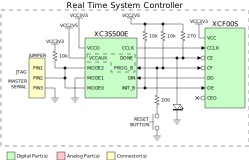
\includegraphics{./figures/Config} 
	\caption{Connection of the Platform FLASH Configuration PROM to the FPGA~\cite{DigilentNexys2rm,DigilentNexys2sch}\label{fig:Config}}
\end{figure}

There are three pins on the FPGA that control the configuration mode.  These pins are labeled MODE[0:2].  The FPGA is capable of several configuration modes, but the modes available on the RTSC are shown in Table~\ref{tab:ConfigMode}.

\renewcommand{\arraystretch}{1.3}
\begin{table}[h]
\centering
\begin{tabular}{|l|l|}
\hline
MODE[0:2]& Configuration mode\\
\hline
[0 0 0] & Master Serial (Platform Flash)\\
\hline
[1 0 1] & JTAG Mode\\
\hline
\end{tabular}
\caption{FPGA configuration modes from a table in~\cite{Spartan3ConfigUG}\label{tab:ConfigMode} }

\end{table}
\renewcommand{\arraystretch}{1.0}

\subsubsection{Master Serial}

Xilinx\textsuperscript{\textregistered}  has created a line of flash ICs that make on board configuration very simple.  Using the Platform Flash ICs, the Spartan 3E FPGA can configure itself in Master Serial mode where the FPGA controls the serial data clock and enables the flash chip~\cite{Spartan3ConfigUG}.  The XCF04S 4Mbit Platform Flash device provides enough storage for one configuration file for the XC3S500E~\cite{Spartan3ConfigUG}.

Upon power up, the INIT\textunderscore B and DONE open-drain IO pins and the PROG\textunderscore B input pin are pulled high.  INIT\textunderscore B going high causes the FPGA to sample the MODE[0:2] pins, and if Master Serial is the mode selected, INIT\textunderscore B is pulled low, resetting the Platform Flash while the configuration is cleared, after which INIT\textunderscore B is allowed to go high.  DONE is pulled low, enabling the Platform Flash, and the FPGA begins to generate a clock on CCLK, causing the Platform Flash to present data on its DO pin.  After configuration is complete, DONE is allowed to go high, and by virtue of the resistor and LED connected to the pin, the LED will turn on and DONE and $\overline{\mathrm{CE}}$ voltage will be at $\unit{V} _ {\unit{F}}$ of the LED~\cite{Spartan3ConfigUG}.

Pulsing PROG\textunderscore B low for at least $500\unit{ns}$ will cause the FPGA to clear the configuration memory, pull INIT\textunderscore B low, and sample the MODE[0:2] pins when INIT\textunderscore B goes high~\cite{Spartan3ConfigUG}.  The reset button on the RTSC will cause the FPGA to clear its configuration and reconfigure itself or wait for the JTAG interface, depending on the status the MODE[0:2] pins.


\subsubsection{JTAG}

A method of testing interconnects between integrated circuits (IC) on a PCB called Boundary Scan is commonly implemented on digital ICs.  The Boundary Scan standard was developed by the Joint Test Action Group (JTAG) and later adopted as an IEEE standard with the designation IEEE Std. 1149.1.  Boundary Scan, which is commonly referred to as JTAG~\cite{CorelisJTAG}.

The JTAG interface also provides in-circuit programming capabilities which is the feature that is used to configure the FPGA, Platform Flash, and CPLD.  Multiple devices can be daisy-chained in a single JTAG interface.  The list of signals is in the Table~\ref{tab:JTAGSigName}, which is based on~\cite{CorelisJTAG}.




%
% Table begins
% 


\renewcommand{\arraystretch}{1.3}
\begin{table}[h]
\centering
\begin{tabular}{|l|l|p{3in}|}
\hline

Abbreviation&

Signal&

Description\\
\hline

TCK&

Test Clock&

Clock signal bussed to all devices in the chain\\
\hline


TMS&

Test Mode Select&

Mode signal bussed to all devices in the chain\\
\hline


TDI&

Test Data In&

Data to be shifted into device JTAG logic from the previous device in the chain.  Sampled on rising edge of TCK\\
\hline


TDO&

Test Data Out&

Data to be shifted out of device JTAG logic to the next device in the chain.  Updated on falling edge of TCK\\
\hline
\end{tabular}
\caption{JTAG signal names and descriptions~\cite{CorelisJTAG}\label{tab:JTAGSigName} }
\end{table}
\renewcommand{\arraystretch}{1.0}

To program the FPGA, Platform Flash, or CPLD, a JTAG programming cable available from Digilent\textsuperscript{\textregistered}, Xilinx\textsuperscript{\textregistered}, or another vendor may be connected to the JTAG header, or the JTAG capabilities of the Cypress microcontroller may be utilized with the Digilent\textsuperscript{\textregistered} ADEPT PC software.  Details of the JTAG connections, which are based on~\cite{DigilentNexys2sch}, are shown in Figure~\ref{fig:JTAGChain}.  The resistors on the TCK, TMS, and XC3S500E TDI lines are required to be $>68\unit{\Omega}$ for $3.3\unit{V}$ JTAG interfaces ($0\unit{\Omega}$ for $2.5\unit{V}$ interface)~\cite{Spartan3ConfigUG}.  Reference~\cite{DigilentNexys2sch} uses $200\unit{\Omega}$ resistors.

\begin{figure}[H]
	\centering 
		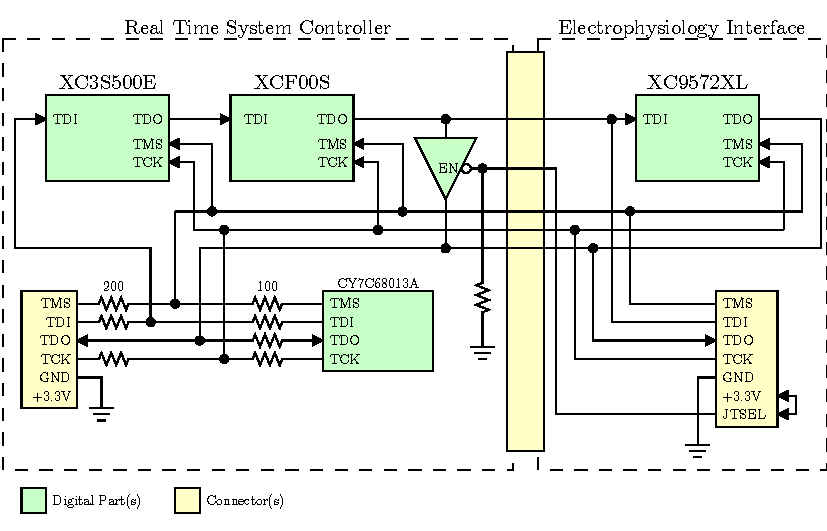
\includegraphics{./figures/JTAGChain} 
	\caption{Signals in the JTAG scan chain; RTSC connections based on~\cite{DigilentNexys2sch}\label{fig:JTAGChain}}
\end{figure}

The RTSC routes the JTAG scan chain through the FPGA, then the Platform Flash, and finally over the Hirose FX2 connector.  If a peripheral board connected to the FX2 connector does not connect to the RTSC's JTAG scan chain, a tri-state buffer, with its active-low output-enable pin pulled low, routes the TDO signal of the Platform Flash to the Cypress microcontroller and JTAG programming cable header.  To enable the CPLD on the Electrophysiology Interface board to be programmed through the JTAG scan chain of the RTSC, the TDO signal from the Platform Flash is routed to the TDI pin of the CPLD, the TDO pin of the CPLD is routed to the Cypress microcontroller and JTAG programming header on the RTSC, and the TMS and TCK signals are bussed to the CPLD.  A header on the Electrophysiology Interface board allows probing of the JTAG signals, or if the board is not connected to the RTSC, a JTAG programming cable may be connected to the header to program the CPLD.  The output-enable pin of the tri-state buffer is routed to the JTSEL signal on the Electrophysiology Interface board.  To prevent the tri-state buffer and CPLD from acting as an output on the same signal, connecting JTSEL to $+3.3\unit{V}$ on the header on the Electrophysiology Interface board will disable the output of the tri-state buffer.  Thus, simply connecting the Electrophysiology Interface board to the RTSC board will put the CPLD in the RTSC's JTAG scan chain.

Steps for configuring the FPGA or CPLD or loading a configuration file into the Platform Flash in JTAG mode:

\begin{enumerate}
	\item Set the configuration jumper on the RTSC to JTAG Mode

	\item If the Electrophysiology Interface board is connected to the RTSC, configure the power supplies so that the CPLD's VCC and VCCIO pins will be powered

	\item Connect the USB cable to the RTSC, or connect the JTAG programming cable to the JTAG header on the RTSC

	\item Turn on power to the RTSC and Electrophysiology Interface, if it's connected

	\item Follow the steps required in the PC software for the programming cable to load the configuration file onto the FPGA, Platform Flash, or CPLD
\end{enumerate}
